\section{Интерполирование кривой по набору точек}

На рис.~\ref{picture-by-points-plane} изображена сплайн-кривая на плоскости, построенная по набору точек. Можно видеть,
что две средние точки соединены участками окружностей. Также здесь наглядно показан результат деформации одной кривой
в другую, "--- это участок результирующей кривой, соединяющий две средние точки.

\begin{figure}[h!]
\center{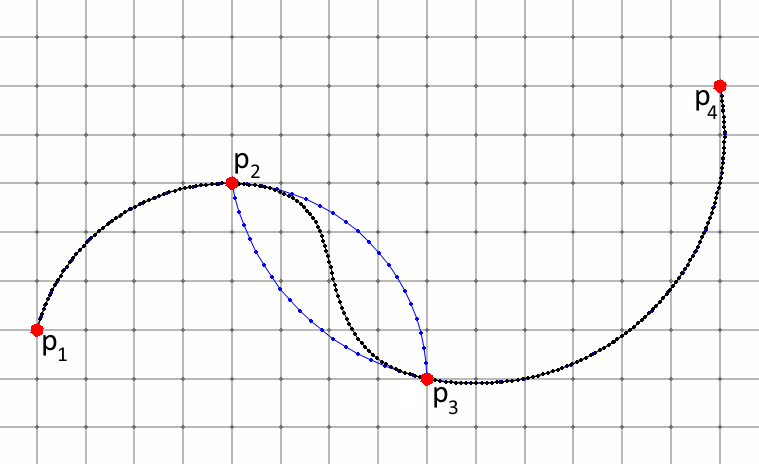
\includegraphics[scale=0.7]{by-points-plane}}
\caption{Интерполирование кривой по набору точек на плоскости}
\label{picture-by-points-plane}
\end{figure}

На рис.~\ref{picture-by-points-two-dimension} изображена сплайн-кривая на поверхности двумерной сферы, построенная
по набору точек. Здесь, по аналогии с предыдущим изображением, можно видеть, что две средние точки соединены между собой
участками двух различных малых дуг. Также наглядно показан результат деформации одной малой дуги в другую.

\begin{figure}[h!]
\center{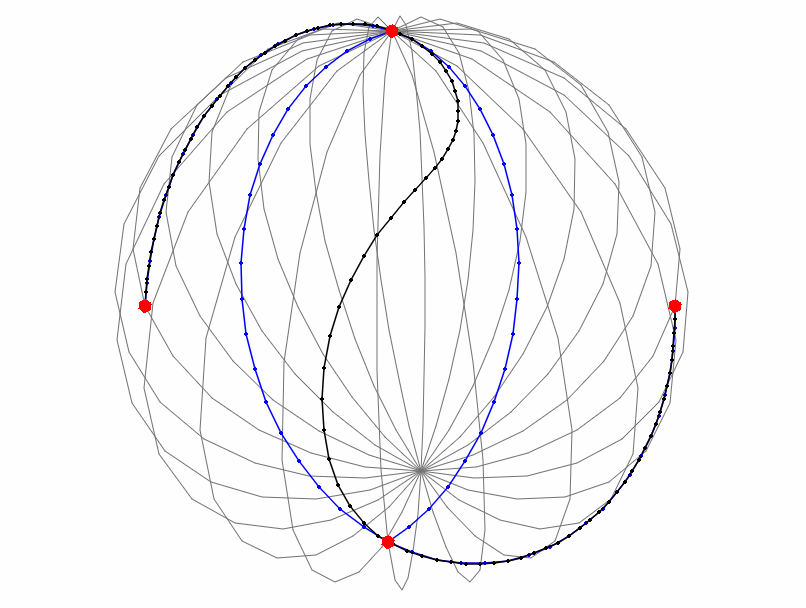
\includegraphics[scale=0.7]{by-points-two-dimension}}
\caption{Интерполирование кривой по набору точек на двумерной сфере}
\label{picture-by-points-two-dimension}
\end{figure}

На рис.~\ref{picture-by-points-orientation} можно видеть набор ориентаций 3D-объекта. Чёрным выделен объект
в изначальном положении. Через все остальные ориентации этот объект должен пройти последовательно. Чёрная
кривая "--- это тот путь, который пройдёт самая верхняя точка объекта при воспроизведении построенной анимации.

\begin{figure}[h!]
\center{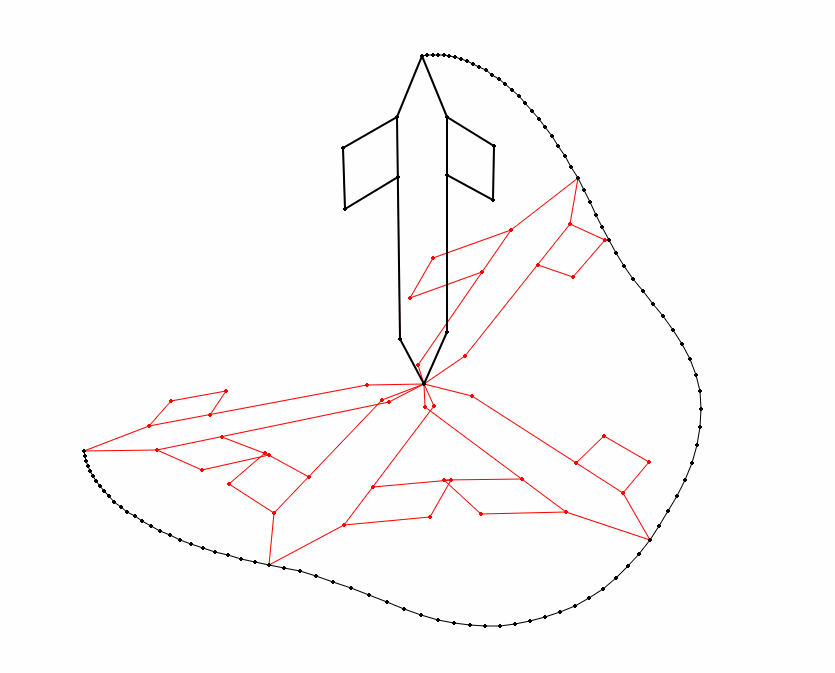
\includegraphics[scale=0.8]{by-points-orientation}}
\caption{Интерполирование кривой по набору точек на ориентационной сфере}
\label{picture-by-points-orientation}
\end{figure}
